\documentclass[final,hyperref={pdfpagelabels=false}]{beamer}
\usepackage{grffile}
\mode<presentation>{\usetheme{I6pd2}}
\usepackage[english]{babel}
\usepackage[latin1]{inputenc}
\usepackage{amsmath,amsthm, amssymb, latexsym}
\usepackage{tikz}
\usetikzlibrary{shapes.geometric, arrows,backgrounds,fit}
\usepackage{booktabs}
\usepackage{caption}
\captionsetup{justification={justified}}
\usepackage[square,numbers]{natbib}
\usepackage{ragged2e}
\tikzstyle{arrow} = [thick,line width=0.8mm,->,>=stealth]
\usepackage{hyperref}

%\usepackage{times}\usefonttheme{professionalfonts}  % obsolete
%\usefonttheme[onlymath]{serif}
\boldmath
\usepackage[orientation=portrait,size=a0,scale=1.4,debug]{beamerposter}
% change list indention level
% \setdefaultleftmargin{3em}{}{}{}{}{}


%\usepackage{snapshot} % will write a .dep file with all dependencies, allows for easy bundling

\usepackage{array,booktabs,tabularx}
\newcolumntype{Z}{>{\centering\arraybackslash}X} % centered tabularx columns
\newcommand{\pphantom}{\textcolor{ta3aluminium}} % phantom introduces a vertical space in p formatted table columns??!!
\setbeamercolor{background canvas}{bg=lightgray}
\setbeamercolor*{block body}{bg=white, fg=black}
\listfiles
%%%%%%%%%%%%%%%%%%%%%%%%%%%%%%%%%%%%%%%%%%%%%%%%%%%%%%%%%%%%%%%%%%%%%%%%%%%%%%%%%%%%%%
\graphicspath{{figures/}}
 
\title{
\huge Collaborative Text Filtering}
\author{Peter J. Bakke (s183268), Daniel Horvath (s172185), Christian Hansen (s146498) and Thomas Brenner (s181857)}
\institute[Department]{\small DTU Compute, Technical University of Denmark}
\date[December. 17th, 2018]{December. 17th, 2018}

%%%%%%%%%%%%%%%%%%%%%%%%%%%%%%%%%%%%%%%%%%%%%%%%%%%%%%%%%%%%%%%%%%%%%%%%%%%%%%%%%%%%%%
\newlength{\columnheight}
\setlength{\columnheight}{105cm}

\begin{document}

\begin{frame}
 \begin{columns}
% ---------------------------------------------------------%
% Set up  COLUMN 1
% ---------------------------------------------------------%
 \begin{column}{.49\paperwidth}
 \begin{beamercolorbox}[center,wd=\textwidth]{postercolumn}
 \begin{minipage}[T]{.99\textwidth}  % tweaks the width, makes a new \textwidth
 \parbox[t][\columnheight]{\textwidth}{ % must be some better way to set the the height, width and textwidth simultaneously
                                                            % Since all columns are the same length, it is all nice and tidy.  You have to get the height empirically

% ---------------------------------------------------------%
% set up block  INTRODUCTION
% ---------------------------------------------------------%
\begin{block}{Introduction}
 \begin{columns}
 \begin{column}{1\textwidth}



\centering
\begin{minipage}[t]{0.98\textwidth}

\footnotesize{Collaborative text filtering is one of the most popular and effective approaches for recommender systems. Recommender systems are based on the idea, that given previously collected data about users and their interactions with items, you can predict whether a given user wants to have an interaction with a given item. This is widely used for platforms like Netflix, Amazon, Youtube and news websites. These platforms can increase their profits by being able to predict their consumers interests and showing content relevant for the user. 

The purpose of this project is to match two text descriptions of varied lengths. More concretely we propose a model to recommend articles to users based on the abstracts from other articles a user has indicated as read.
\vspace{0.5cm}
}



\end{minipage} \hspace{1cm}


      
\end{column}
 \end{columns}
 \end{block}
 \vfill


% ------------------------------------------------
% set up block METHODOLOGY
% ------------------------------------------------

\begin{block}{General Methodology}
 \begin{columns}
 \begin{column}{1\textwidth}


\centering
\begin{minipage}[t]{0.98\textwidth}

\footnotesize{
In general we try to maximize the probability of a match between a user and an item given some features: 
%
\begin{align*}
\max p (m | K; \theta)
\end{align*}
%
where $m$ denotes the binary variable on whether there is match, $K$ denotes the features, and $\theta$ denotes the parameters in the model.

To predict a users preferences we use
%
%
\begin{align*}
    p(m) = \sigma( f ( \text{UserId, MovieId}) ) 
\end{align*}
%
where $\sigma( \cdot )$ denotes the sigmoid function and $f( \cdot )$ is some function of users and items. In the matrix factorization $f(\cdot)$ could be given by the inner product of embeddings of users and items, e.g.:
%
%
\begin{align*}
    f(\cdot) = u \cdot m^T
\end{align*}
%
%
where
%
%
\begin{align*}
    u &= \text{Embedding}(x_u) \\
    m &= \text{Embedding}(x_m) 
\end{align*}
%
%
When we turn to the more advanced models $f(\cdot)$ is e.g. a neural net or LSTM net with user/item embeddings as input features instead of a simple inner product between the two, \cite{paragraph_embedding_comparison, Embedding, doc2vec}.
\vspace{0.5cm}
}



\end{minipage} \hspace{1cm}


      
\end{column}
 \end{columns}
 \end{block}
 \vfill

% ---------------------------------------------------------%
% set up block  DATA
% ---------------------------------------------------------%

 \begin{block}{Data}
 \begin{columns}
 \begin{column}{1\textwidth}
 


\vspace{-0.5cm}

\begin{minipage}[t]{0.98\textwidth}
\begin{itemize}
\justifying
\footnotesize{
        \item We use the publicly available \textbf{MovieLens} dataset from \url{https://grouplens.org/datasets/movielens/} for the first part of our project
	\item We use the publicly available \textbf{CiteULike} from \url{http://www.citeulike.org/faq/data.adp} for the second part of our project
}
\end{itemize}


\end{minipage} 



\vspace{0.5cm}

					
          
\end{column}
\end{columns}
\vskip-1ex
\end{block}
\vfill



% ---------------------------------------------------------%
% set up block  DATA
% ---------------------------------------------------------%

 \begin{block}{Key points}
 \begin{columns}
 \begin{column}{1\textwidth}
 


\vspace{-0.5cm}

\begin{minipage}[t]{0.98\textwidth}
\begin{itemize}
\justifying
\footnotesize{
        \item We construct a baseline model using \textbf{Matrix Factorization} on the MovieLens and CiteUlike datasets
	\item We construct a \textbf{Collaborative Text Filtering} model on the same data using
	{\setbeamertemplate{itemize items}[ball]
	\begin{itemize}
	\footnotesize{
	\item  \quad Feed Forward Networks, \cite{ncf2017, nielsenneural} 
	\item  \quad LSTM Networks, \cite{lstm1997}}
	\end{itemize}}
	And compare the results to the baseline model, \cite{lcmr2018, itemBasedCF2001, HU2008CollaborativeFF}
	\item We implement the models using the \textbf{Pytorch} deep learning framework and use \textbf{TorchText} for creating word embeddings and batch iterators
	\item We train the models using virtual machines on the \textbf{Google Colab} GPU cloud
}
\end{itemize}


\end{minipage} 
%\end{minipage} \hspace{1cm} \begin{minipage}[t]{.5\textwidth}


\vspace{0.5cm}

					
          
\end{column}
\end{columns}
\vskip-1ex
\end{block}
\vfill




% ---------------------------------------------------------%
% set up block  MovieLens
% ---------------------------------------------------------%


 \begin{block}{MovieLens}
 \begin{columns}
 \begin{column}{1\textwidth}


%\vspace{0.5cm}

\centering
\begin{minipage}[t]{0.96\textwidth}
			

\hspace{0.5cm} 
\vspace{-1cm}
\begin{columns}
 \begin{column}{0.45\textwidth}
 \justifying
 \footnotesize{
	The MoveieLens dataset consist of 20 million ratings on a scale from 0.5 to 5, of 27,000 different movies by 138,000 users. Taking outset in the MovieLens dataset the objective is to predict how a specific user will rate a specific movie. }
 \end{column}
 \begin{column}{0.49\textwidth}

\begin{table}[h]
\small
\centering
\caption{Results} 
\label{res:MovieLens_results}
\begin{tabular}{lrrr}
\toprule
Model  & Best accuracy        & Best Epoch     & Something else    \\
\midrule
MF  	&  0.1337        & 2       & 0.1337    \\
FNN	  &  0.1337        & 12      & 0.1337    \\
\bottomrule
\end{tabular}
\end{table}

 \end{column}
 \end{columns}
 
 \begin{figure}

\includegraphics[width=0.75\textwidth]{movielensnet.png}
 \caption{MovieLens neural net representation}
\end{figure}  

 \begin{figure}

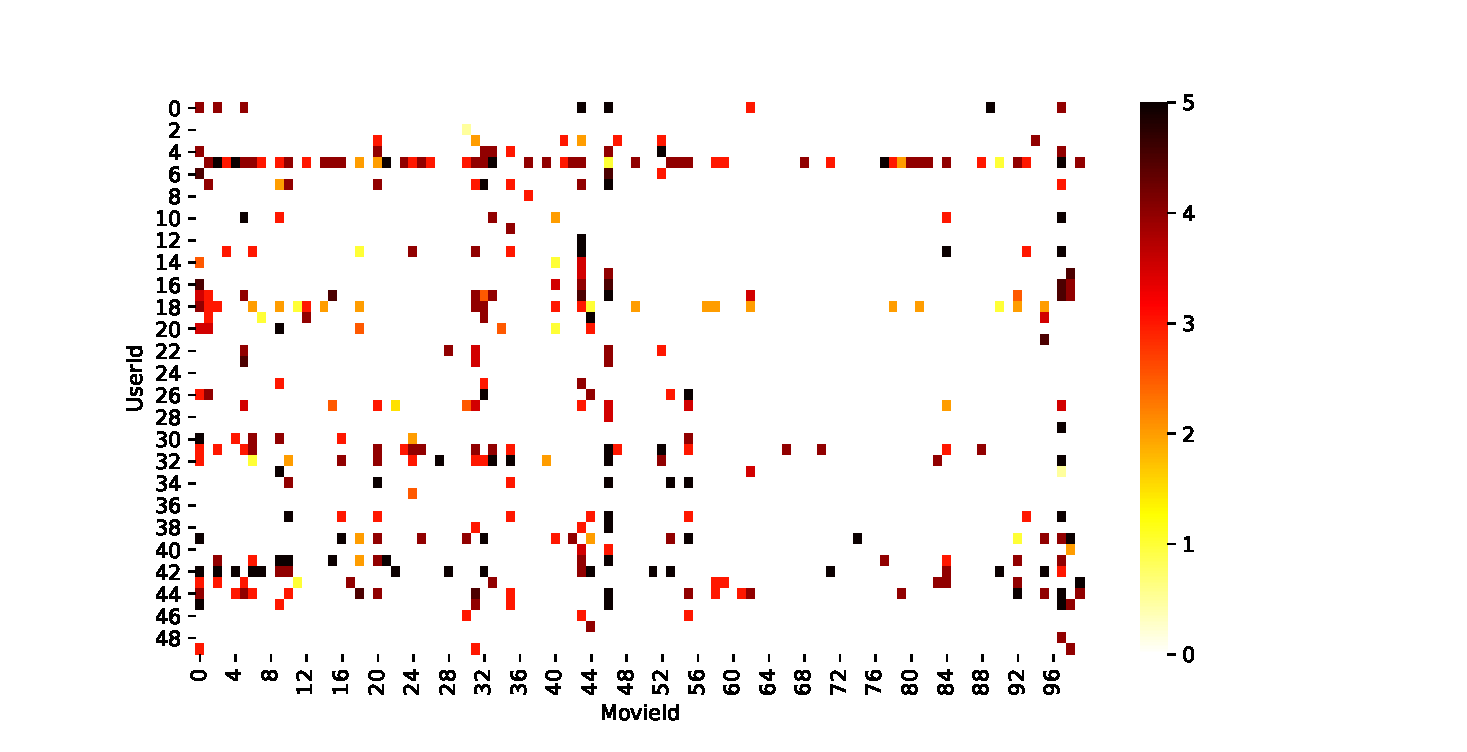
\includegraphics[width=0.49\textwidth]{MovieLens_ratings_true.eps}
 \caption{MovieLens ratings for the first 50 users and 100 movies. The data has been padded with zeroes for all user-movie combinations that have not been given an explicit rating}
\end{figure}  

\end{minipage}



\vspace{0.5cm}

					
                  
\end{column}
\end{columns}
\vskip-1ex
\end{block}
\vfill





}
\end{minipage}
\end{beamercolorbox}
\end{column}
% ---------------------------------------------------------%
% end the COLUMN 1
% ---------------------------------------------------------%
 

% ---------------------------------------------------------%
% Set up COLUMN 2
% ---------------------------------------------------------%
    
\begin{column}{.49\paperwidth}
\begin{beamercolorbox}[center,wd=\textwidth]{postercolumn}
\begin{minipage}[T]{.99\textwidth} % tweaks the width, makes a new \textwidth
\parbox[t][\columnheight]{\textwidth}{ % must be some better way to set the the height, width and textwidth simultaneously
            											% Since all columns are the same length, it is all nice and tidy.  You have to get the height empirically
            

 \begin{block}{CiteULike}
 \begin{columns}
 \begin{column}{1\textwidth}


\centering
\begin{minipage}[t]{0.96\textwidth}
			

\hspace{0.5cm} 
\vspace{-1cm}
\begin{columns}
 \begin{column}{0.45\textwidth}
 \justifying
 \footnotesize{
	The CiteULike dataset consist of users represented by an Id and articles represented by an Id, the article Title and the article Abstract. The user-article interaction is represented as a binary attribute on whether a specific userId has put an ArticleId in his/her "basket". The modelling aim is to build a model that can recommend articles to users based on what they have previously read. }
 \end{column}
 \begin{column}{0.49\textwidth}

\begin{table}[h]
\small
\centering
\caption{Results} 
\label{res:CuL_results}
\begin{tabular}{lrrr}
\toprule
Model  & Best accuracy        & Best Epoch     & Something else    \\
\midrule
MF  	&  0.1337        & 2       & 0.1337    \\
FNN	  &  0.1337        & 12      & 0.1337    \\
LSTM	&  0.1337        & 24      & 0.1337    \\
\bottomrule
\end{tabular}
\end{table}

 \end{column}
 \end{columns}
 
 \begin{figure}

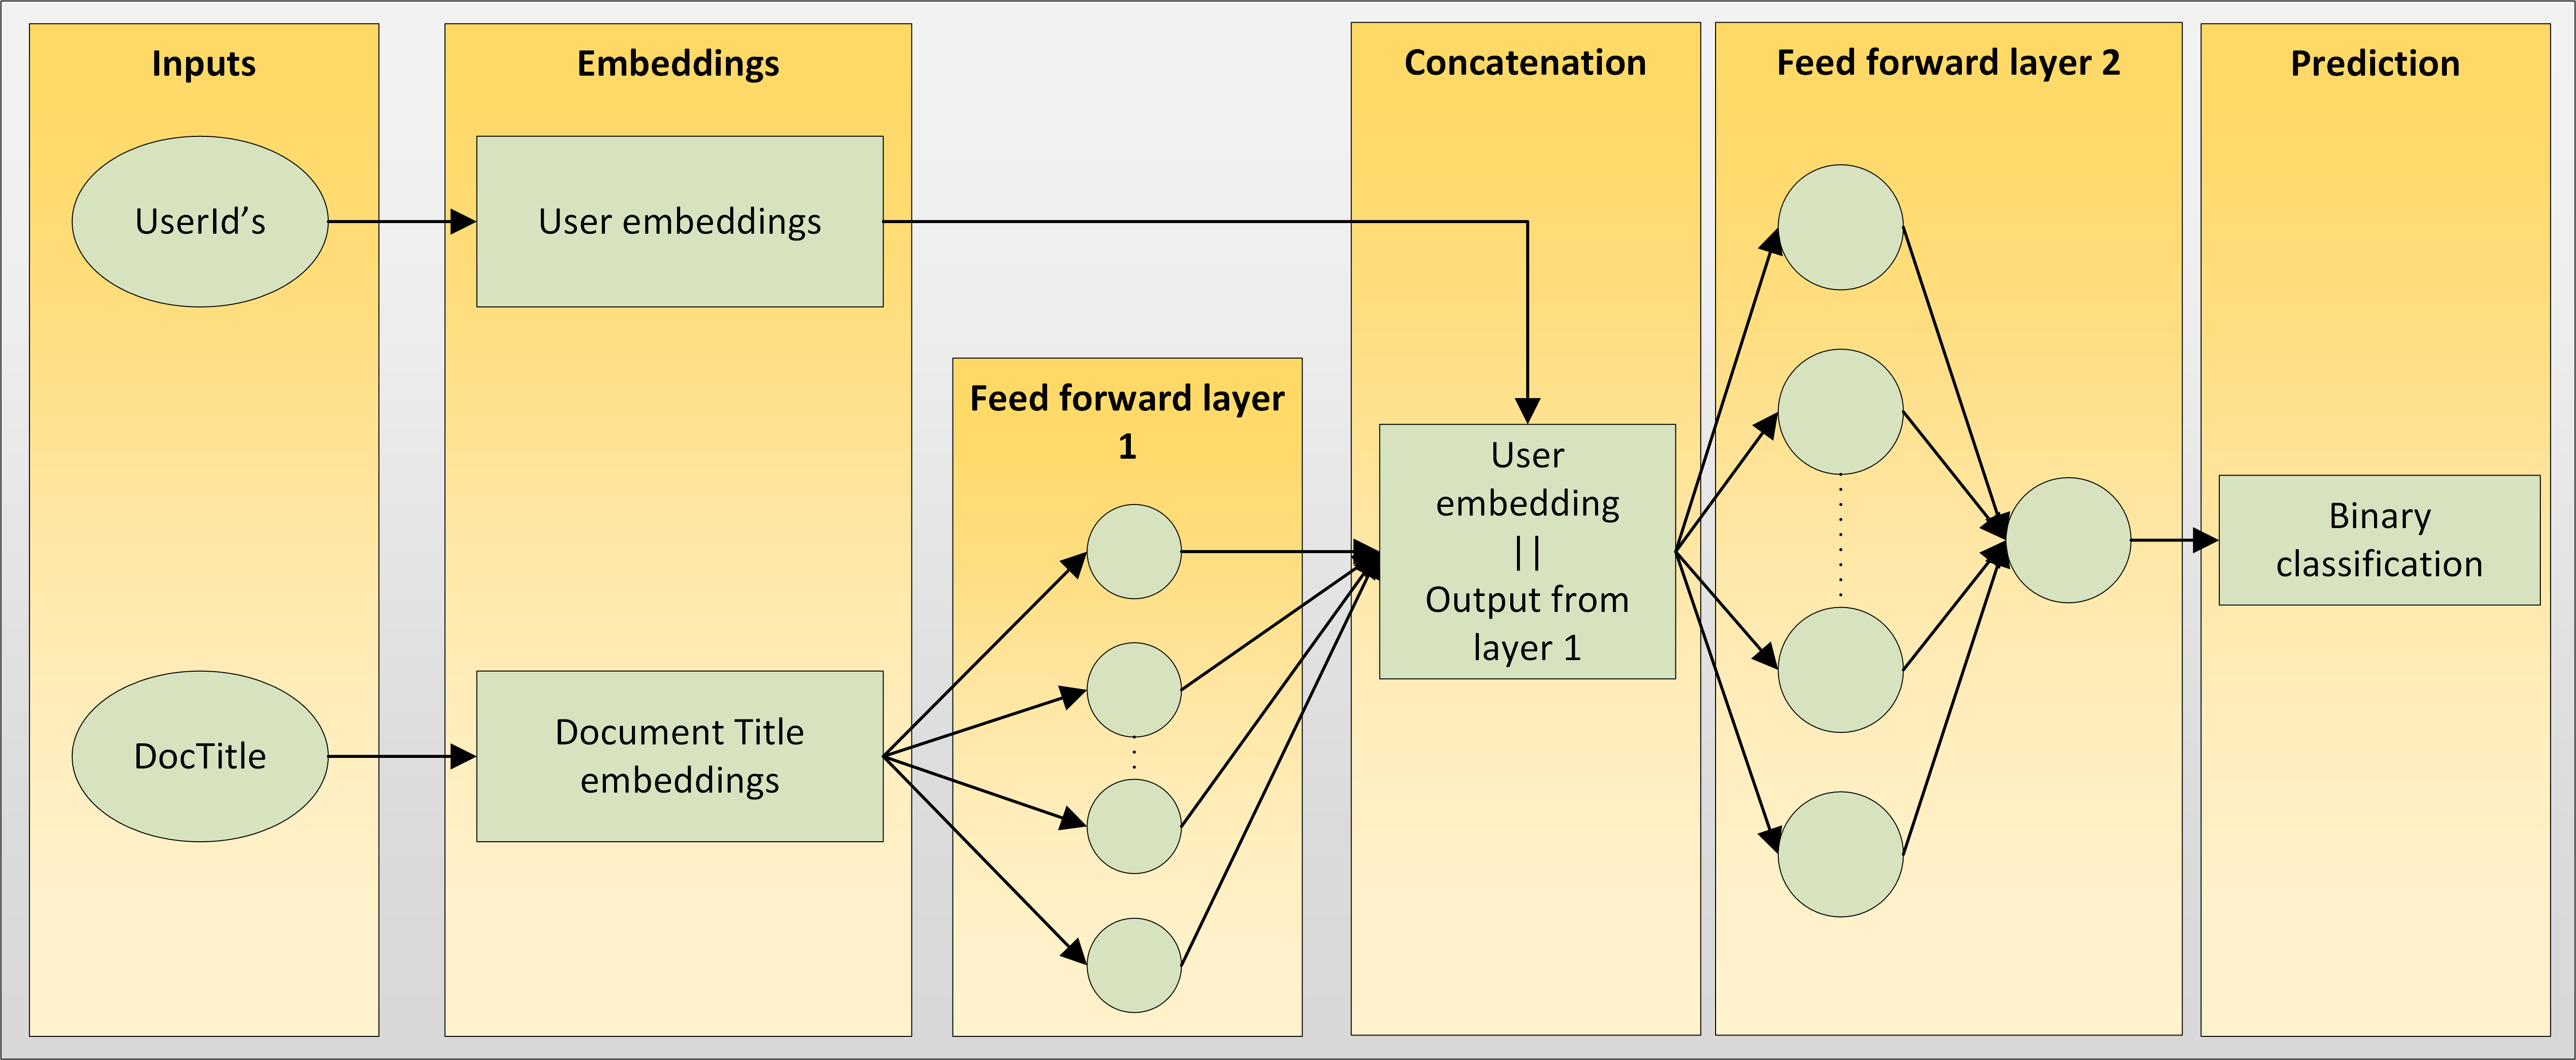
\includegraphics[width=0.85\textwidth]{CiteuLikeNet.png}
 \caption{CiteULike Neural net representation}
\end{figure}  

\begin{figure}

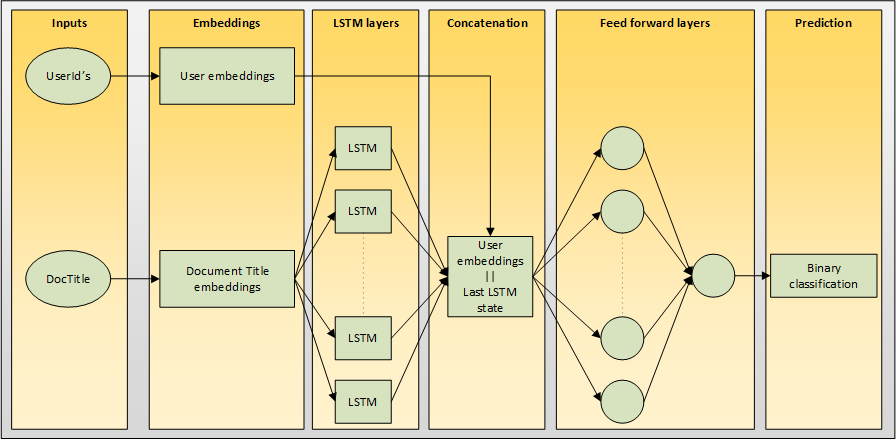
\includegraphics[width=0.85\textwidth]{CiteuLikeLSTM.png}
 \caption{CiteULike LSTM net representation. For clarity the temporal structure of the LSTM blocks have not been shown.}
\end{figure}

\end{minipage}



\vspace{0.5cm}

					
                  
\end{column}
\end{columns}
\vskip-1ex
\end{block}
\vfill	

\begin{block}{Comparison of results}

\begin{columns}
\begin{column}{1\textwidth}

\centering

%\vspace{2.5cm}
\centering
\begin{minipage}[t]{.95\textwidth}


\vspace{-1cm}
\begin{table}[h]
\footnotesize
\caption{Another table to summarize results - or maybe some more charts???}
\begin{tabular}{p{8cm}p{2cm}p{2cm}p{2cm}p{2cm}p{2cm}p{2cm}p{2cm}p{2cm}p{2cm}p{2cm}p{2.5cm}p{2.5cm}}
\toprule
Location      & \multicolumn{10}{l}{What can we possibly show???}        & another metric & AUC or??? \\
\midrule
MovieLens MF          & 680 & 103 & 4   & 5   & 2   & 8   & 1   & 2  & 2 & 1 & 0.842 & 0.784 \\
MovieLens NN         & 94  & 361 &  7  & 18  & 5   & 4   & 3   & 8  & 1 & 7 & 0.711 & 0.608 \\
CuL MF    & 3   & 5   & 365 &  5  & 5   & 4   & 2   & 0  & 4 & 0 & 0.929 & 0.907 \\
CuL NN     & 9   & 21  & 0   & 247 &  0  & 5   & 14  & 2  & 1 & 3 & 0.818 & 0.812 \\
CuL LSTM     & 5   & 15  & 6   & 1   & 203 & 20  & 1   & 4  & 18& 0 & 0.744 & 0.732 \\
\bottomrule

\end{tabular}
\end{table}


\end{minipage}

\end{column}
\end{columns}
\end{block}

\vfill


\begin{block}{Acknowledgements}
\centering
\begin{minipage}[t]{0.98\textwidth}

\footnotesize{The authors wish to thank Alexander R. Johansen and Jose Juan Almagro Armenteros from DTU Lyngby for their constructive feedback and fruitful discussions during the process of the project.}
\end{minipage}
\end{block}
\vfill
\begin{block}{References}

{\scriptsize
\bibliographystyle{abbrvnat}	
\bibliography{biblio}
}			
\end{block}
\vfill


         
}
\end{minipage}
\end{beamercolorbox}
\end{column}
\end{columns}	
% ---------------------------------------------------------%
% end the COLUMN 2
% ---------------------------------------------------------%
  
  
\vskip1ex
%\tiny\hfill\textcolor{ta2gray}{Created with \LaTeX \texttt{beamerposter}  \url{http://www-i6.informatik.rwth-aachen.de/~dreuw/latexbeamerposter.php}}
\tiny\hfill{Created with \LaTeX \texttt{beamerposter}  \url{http://www-i6.informatik.rwth-aachen.de/~dreuw/latexbeamerposter.php} \hskip1em}
\end{frame}
\end{document}